\documentclass[tikz, border=1mm]{standalone}

\usepackage{pgfplots}
\pgfplotsset{compat=1.15}
\usepackage{mathrsfs}
\usepackage{amsfonts}
\usetikzlibrary{arrows}
\pagestyle{empty}


\begin{document}

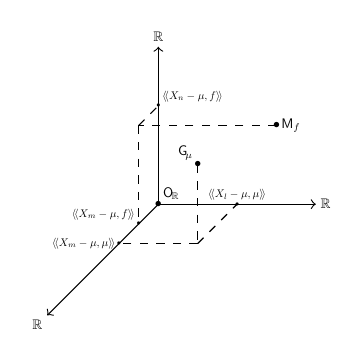
\begin{tikzpicture}

% Write
% \node[draw] at (-1.5, 2) {$\mathcal{G}$};

% Axis
\draw[->] (0, 0) -- (2, 0);
\draw (2, 0) node[right, scale=0.5] {$\mathbb{R}$};

\draw[->] (0, 0) -- (0, 2);
\draw (0, 2) node[above, scale=0.5] {$\mathbb{R}$};

\draw[->] (0, 0) -- (-1.412, -1.412);
\draw (-1.412, -1.412) node[below left, scale=0.5] {$\mathbb{R}$};

% Points
\draw (0, 0) node[scale=0.5] {$\bullet$};
\draw (0, 0) node[above right, scale=0.5] {$\mathsf{O}_{\!\mathbb{R}}$};

\draw (1.5, 1) node[scale=0.5] {$\bullet$};
\draw (1.5, 1) node[right, scale=0.5] {$\mathsf{M}_f$};

\draw (0.5, 0.5) node[scale=0.5] {$\bullet$};
\draw (0.5, 0.5) node[above left, scale=0.5] {$\mathsf{G}_{\!\mu}$};

\draw (1, 0) node[scale=0.3] {$\bullet$};
\draw (1, 0) node[above, scale=0.4] {$\langle\!\langle X_l - \mu, \mu \rangle\!\rangle$};

\draw (-0.5, -0.5) node[scale=0.3] {$\bullet$};
\draw (-0.5, -0.5) node[left, scale=0.4] {$\langle\!\langle X_m - \mu, \mu \rangle\!\rangle$};


\draw (-0.25, -0.25) node[scale=0.3] {$\bullet$};
\draw (-0.25, -0.25) node[above left, scale=0.4] {$\langle\!\langle X_m - \mu, f \rangle\!\rangle$};

\draw (0, 1.25) node[scale=0.3] {$\bullet$};
\draw (0, 1.25) node[above right, scale=0.4] {$\langle\!\langle X_n - \mu, f \rangle\!\rangle$};



% Limes
% \draw[->, >=latex] (0, 0) -- (1, 0.8);
% \draw[->, >=latex] (0, 0) -- (0.3, 1.05);

% For G
\draw[dashed] (0.5, 0.5) -- ++(0, -1);
\draw[dashed] (0.5, -0.5) -- ++(-1, 0);
\draw[dashed] (0.5, -0.5) -- ++(0.5, 0.5);

% For M_i
\draw[dashed] (1.5, 1) -- ++(-1.75, 0);
\draw[dashed] (-0.25, 1) -- ++(0, -1.25);
\draw[dashed] (-0.25, 1) -- ++(0.25, 0.25);


% Arc
% \draw (0.31, 0.25) arc (20:87:0.225);
% \draw (0.29, 0.3) node[above, scale=0.5] {$\theta_{ij}$};

% Cloud
% \draw[rotate around={45:(0, 0)}] (0, 0) ellipse (1.8cm and 1cm);
% \draw (0.2, -1.4) node[above, scale=0.5] {$\mathcal{C}$};

% Distance


\end{tikzpicture}

\end{document}